\usetikzlibrary{calc}
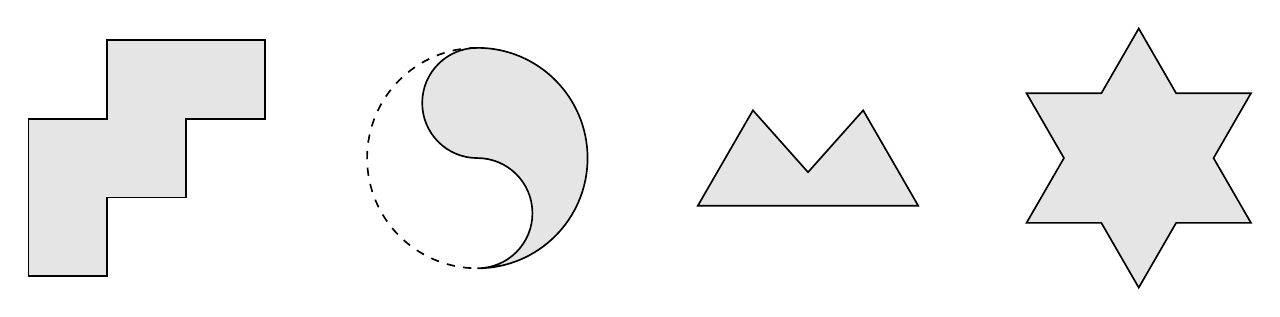
\begin{tikzpicture}[x=1cm,y=1cm,font=\normalsize,
  region edge/.style={solid,line width=.6pt}]
  % panel 1: five-cell staircase polygon, row widths 1,2,2, top row shifted right
  \coordinate (P1a) at (-1.5,-1.5);
  \coordinate (P1b) at (-0.5,-1.5);
  \coordinate (P1c) at (-0.5,-0.5);
  \coordinate (P1d) at (0.5,-0.5);
  \coordinate (P1e) at (0.5,0.5);
  \coordinate (P1f) at (1.5,0.5);
  \coordinate (P1g) at (1.5,1.5);
  \coordinate (P1h) at (-0.5,1.5);
  \coordinate (P1i) at (-0.5,0.5);
  \coordinate (P1j) at (-1.5,0.5);
  \filldraw[region edge,fill=gray!20]
    (P1a)--(P1b)--(P1c)--(P1d)--(P1e)--(P1f)--(P1g)--(P1h)--(P1i)--(P1j)--cycle;

  % panel 2: yin-yang region, outer radius 1.4, inner radius 0.7
  \coordinate (Y2) at (4.2,0);
  \coordinate (Y2t) at (4.2,1.4);
  \coordinate (Y2b) at (4.2,-1.4);
  \filldraw[region edge,fill=gray!20] (4.2,1.4)
    arc[start angle=90,end angle=-90,radius=1.4]
    arc[start angle=-90,end angle=90,radius=0.7]
    arc[start angle=270,end angle=90,radius=0.7];
  \draw[region edge,dashed] (4.2,1.4)
    arc[start angle=90,end angle=270,radius=1.4];

  % panel 3: two equilateral triangles sharing the bottom vertex
  \coordinate (T3L) at (7.0,-0.606217782);
  \coordinate (T3S) at (8.4,-0.606217782);
  \coordinate (T3R) at (9.8,-0.606217782);
  \coordinate (T3A) at (7.7,0.606217782);
  \coordinate (T3B) at (9.1,0.606217782);
  \filldraw[region edge,fill=gray!20] (T3L)--(T3R)--(T3B)--(8.4,-0.18)--(T3A)--cycle;
  

  % panel 4: six-pointed star with 12 equal boundary edges
  \coordinate (S1) at (12.6,1.645448267);
  \coordinate (S2) at (13.075,0.822724134);
  \coordinate (S3) at (14.025,0.822724134);
  \coordinate (S4) at (13.55,0);
  \coordinate (S5) at (14.025,-0.822724134);
  \coordinate (S6) at (13.075,-0.822724134);
  \coordinate (S7) at (12.6,-1.645448267);
  \coordinate (S8) at (12.125,-0.822724134);
  \coordinate (S9) at (11.175,-0.822724134);
  \coordinate (S10) at (11.65,0);
  \coordinate (S11) at (11.175,0.822724134);
  \coordinate (S12) at (12.125,0.822724134);
  \filldraw[region edge,fill=gray!20]
    (S1)--(S2)--(S3)--(S4)--(S5)--(S6)--(S7)--(S8)--(S9)--(S10)--(S11)--(S12)--cycle;
\end{tikzpicture}
